\documentclass[a4paper,man,natbib,11pt]{article}
\textwidth=7in
\textheight=9.5in
\topmargin=-1in
\headheight=0in
\headsep=.5in
\hoffset  -.85in

\usepackage[english]{babel}
\usepackage[utf8x]{inputenc}
\usepackage{amsmath}
\usepackage{setspace}
\usepackage{graphicx}
\usepackage{longtable}
\usepackage{graphicx}
\usepackage{caption}
\usepackage{subcaption}
%\usepackage{apacite}
\usepackage{tikz}
\usetikzlibrary{positioning,arrows.meta,quotes}
\doublespacing
%\usepackage{lineno}
%\linenumbers
\title{Predicting Dementia using Machine Learning Methods}
\author{Peter Shewmaker, Nadia Mercado,Caroline Mills  }
\date{April 2020}

\begin{document}

\maketitle

\section{Introduction}

Dementia and other cognitive decline diseases are a serious financial and medical global concern. As such, in this paper we will test statistical classification methods from statistical learning methods, logistic regression, support vectors machines, and naive baye's. We will present the classification accuracy, specificity, sensitivity, and area under the ROC curve for all classifier methods. 

\section{Data}

The data was drawn from the National Alzheimer's Coordinating Center's Uniform Data Set. Located at the University of Washington, the National Alzheimer's Coordinating Center (NACC) was founded in 1999 by the National Institute on Aging, a division of the National Institutes of Health. The goal of the NACC is to develop and maintain databases of Alzheimer's related research data. The NACC Uniform Data Set is intended to be "the first and primary resource for researchers analyzing NACC clinical and demographic data".

The data contains one row for each clinic visit by a patient. It includes social, racial, educational demographic data, as well as cognitive test results, living situation, and smoking status. In order to use the data for the classification of dementia status, the last recorded visit by each patient included in the data was extracted.

\section{Classification by Test Scores}

Diagnosis of Alzheimer's disease and related dementias is often aided by the use of cognitive tests. The Uniform Data Set contains patient performance on a large variety of these cognitive tests. Some of these tests are owned by private companies or can only be administered by a medical professional. However, other tests could be simply administered by a loved one. 

The aim then was to develop a statistical learning model that could take in patient demographic information together with simple test score results that could theoretically be used for a home screening test for Alzheimer's diagnosis. Cognitive tests were chosen as predictors if they could be administered simply at home. 

Some of the cognitive tests chosen include: Logical Memory, which measures the number of components of a story a patient recalls immediately after being told the story. In the Animal/Vegetable test, the subject is asked to name as many animals (vegetables) as possible in 60 seconds. The Digit Span test involves giving a sequence of digits to a patient and asking them to repeat them, both in the forwards and backwards direction of the original sequence. The Trails test consists of a set of numbered (lettered) dots, and the patient is asked to connect the dots in numerical (alphabetical) order, the test is measured by the amount of time needed to complete the task.

\subsection{Classification Tree}

The first model used to classify patient's dementia status was a classification tree. Of the 7,685 rows in the original data, 46 rows were excluded due to missing data. Then, of the remaining 7,639 rows, 5,000 were selected to form the training data. The remaining 2,639 rows were set aside to be the test set.

\begin{figure}
\centering
\begin{subfigure}{.5\textwidth}
  \centering
  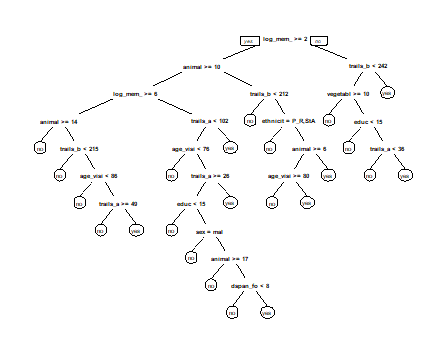
\includegraphics[width=\linewidth]{unpruned_tree.png}
  \caption{Unpruned Tree}
  \label{fig:sub1}
\end{subfigure}%
\begin{subfigure}{.5\textwidth}
  \centering
  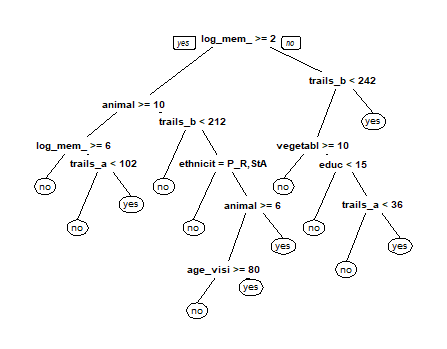
\includegraphics[width=\linewidth]{pruned_tree.png}
  \caption{Pruned Tree}
  \label{fig:sub2}
\end{subfigure}
\caption{Unpruned and Pruned Classification Trees}
\label{fig:test}
\end{figure}

The classification tree was created using the "rpart" package in R. Splits in the tree were made by the Gini index. The complexity parameter was chosen by repeated cross validation. The cross validation was performed using the R package "caret".

In Figure 1 you can see graphical depictions of both the pruned and unpruned trees. The tree was pruned by classification error. We see that the Logical Memory, Trails, and Animal/Vegetable tests are commonly chosen as places to split the tree.

\begin{figure}
\centering
\begin{subfigure}{.5\textwidth}
  \centering
  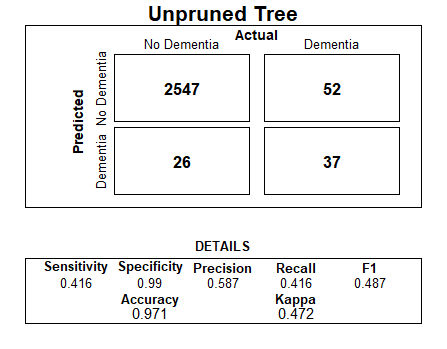
\includegraphics[width=\linewidth]{unpruned_confusion.png}
\end{subfigure}%
\begin{subfigure}{.5\textwidth}
  \centering
  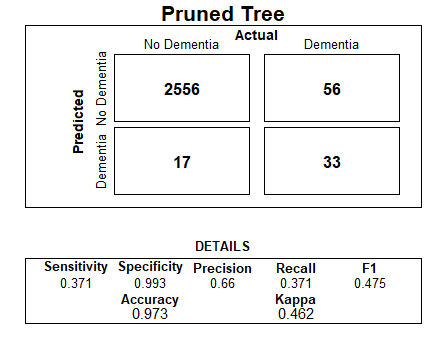
\includegraphics[width=\linewidth]{pruned_confusion.png}
\end{subfigure}
\caption{Unpruned and Pruned Classification Tree Results}
\label{fig:test}
\end{figure}

The comparison of the confusion matrices of the results of the unpruned and pruned tree can be found in Figure 2. We see that the accuracy of the tree was slightly improved after pruning. However, we see that the pruned tree has a lower sensitivity, and classifies correctly fewer of the patients who actually have dementia. 

\subsection{Random Forest with Downsampling}

Though the accuracy of each of the trees appears quite high, it is artificially inflated by the imbalance of the classes. Of the 2639 patients in the testing set, only 89 actually have Alzheimer's, which is 3.3\% of the test set. Therefore a decision tree that classified everyone as not having dementia would have a 96.7\% accuracy! 

Therefore we would like the model used to account for the unbalanced classes. We also see that the trees created in the previous section have a very low sensitivity, which would make it a poor diagnostic screening tool. By accounting for the unbalanced classes, we hope to improve the sensitivity of the classifier.

The method I used to account for the unbalanced classes is called \textit{downsampling}. In a downsampled random forest, instead of using a bootstrap sample from the entire training data set to create each tree, a bootstrap sample from the rare class is generated and a sample of the same size is generated from the common class are joined and used for the creation of the tree. Therefore each tree in the random forest model is built from a data set with the same number of observations in each class.

For some other statistical learning algorithms, the use of downsampling would require getting rid of a large amount of the data. However, since random forest uses resampling, the downsampling can be applied while still making use of the entirety of the training set.

\begin{figure}
\centering
\begin{subfigure}{.5\textwidth}
  \centering
  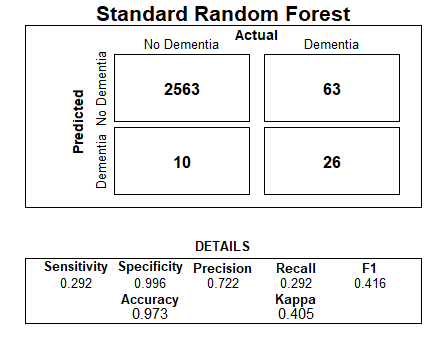
\includegraphics[width=\linewidth]{standard_rf.png}
\end{subfigure}%
\begin{subfigure}{.5\textwidth}
  \centering
  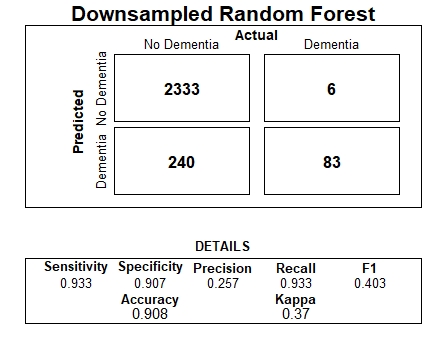
\includegraphics[width=\linewidth]{downsampled_rf.png}
\end{subfigure}
\caption{Standard and Downsampled Random Forest}
\label{fig:test}
\end{figure}

The random forest models were fit using the "caret" package. Cross validation was used to select optimal values for the number of trees and the "mtry" parameter.

The results of both the downsampled and the standard random forest models can be seen in Figure 3. Though the standard random forest model has a much higher accuracy (comparable to the classification trees), the downsampled random forest trades some accuracy for a drastic improvement in sensitivity. The sensitivity and specificity of the downsampled random forest are higher than 0.9, which means that it could be useful as a screening test. The algorithm was able to correctly identify 83 of the 89 patients who did in fact have dementia.

\section{Support Vector Machines}

Support Vector Machine(SVM) is an approach for classification. The e1071 library in R was used to put a SVM to the data. 


\end{document}
